\documentclass[]{BasiliskReportMemo}
\usepackage{AVS}


\newcommand{\submiterInstitute}{Autonomous Vehicle Simulation (AVS) Laboratory,\\ University of Colorado}

\newcommand{\ModuleName}{test\textunderscore unitThrusterDynamics}
\newcommand{\subject}{Sunline EKF Module and Test}
\newcommand{\status}{Initial document}
\newcommand{\preparer}{T. Teil}
\newcommand{\summary}{This module implements and tests a Extended Kalman Filter in order to estimate the sunline direction.}


\begin{document}


\makeCover



%
%	enter the revision documentation here
%	to add more lines, copy the table entry and the \hline, and paste after the current entry.
%
\pagestyle{empty}
{\renewcommand{\arraystretch}{2}
\noindent
\begin{longtable}{|p{0.5in}|p{4.5in}|p{1.14in}|}
\hline
{\bfseries Rev}: & {\bfseries Change Description} & {\bfseries By} \\
\hline
Draft & Initial Revision & T. Teil \\
\hline

\end{longtable}
}

\newpage
\setcounter{page}{1}
\pagestyle{fancy}

\tableofcontents
~\\ \hrule ~\\

%\begin{figure}[htb]
%	\centerline{
%	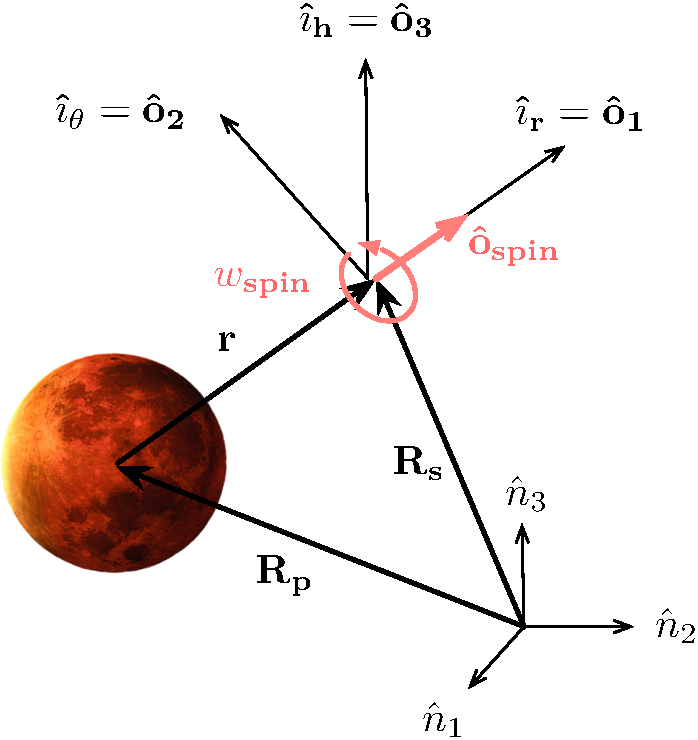
\includegraphics[]{Figures/Fig1}
%	}
%	\caption{Sample Figure Inclusion.}
%	\label{fig:Fig1}
%\end{figure}

\section{Introduction}
The Extended Kalman filter (EKF) in the AVS Basilisk simulation is a sequential
filter implemented to give the best estimate of the desired states.
In this method we estimate the sun heading as well as it's rate of change.
The EKF reads in the message written by the coarse sun sensor, and writes a message 
containing the sun estimate. 

This document summarizes the content of the module, how to use it, and the test that 
was implemented for it.

\begin{figure}[h]
\centering
            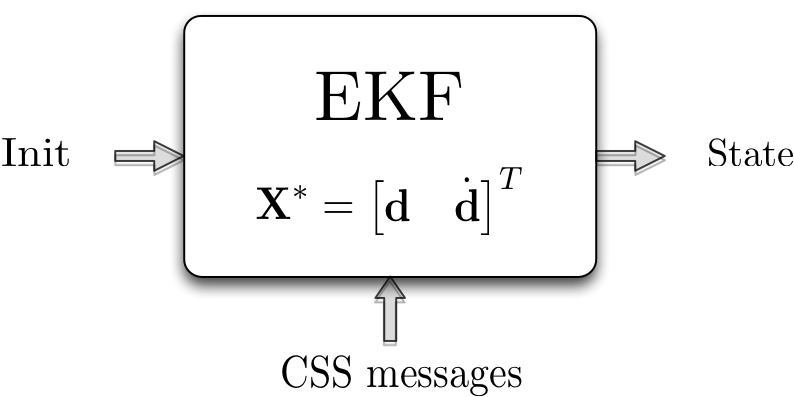
\includegraphics[height=0.3\textwidth,keepaspectratio]{Figures/SchematicEKF.png}
\caption{Filter module}
\end{figure}

\section{Filter Set-up, initialization, and I/O}

\subsection{Dynamics}

The states that are estimated in this filter are the sunline vector, and it's rate of change $\bm X^* = \begin{bmatrix} \bm d &  \dot{\bm d}\end{bmatrix}^T$. The star superscript represents that
this is the reference state. 

The dynamics are given in equation \ref{eq:dyn}. Given the nature of the filter, there is an unobservable state component: the rotation about the $\bm d$ axis. In order to remedy this, we project the states along this axis and subtract them, in order to measure only observable state components. 

\begin{equation}\label{eq:dyn}
\bm F(\bm X) = \begin{bmatrix} \bm F_1(\bm d) \\  \bm F_2(\dot{\bm d})\end{bmatrix} =  \begin{bmatrix} \dot{\bm d} - \left( (\bm d \cdot \dot{\bm d} )\frac{\bm d}{||\bm d||^2} \right) \\ - \frac{1}{\Delta t}\left( (\bm d \cdot \dot{\bm d}) \frac{\bm d}{||\bm d||^2} \right)\end{bmatrix} 
\end{equation}

This leads us to the computation of the dynamics matrix $A = \left[\frac{\partial \bm F (\bm X, t_i)}{\partial \bm X}\right]^{*}$. The partials are given in equation \ref{eq:dynmat}, and were verified in Mathematica.

\begin{align}\label{eq:dynmat}
A&= \begin{bmatrix} \frac{\partial \bm F_1 (\bm X, t_i)}{\partial \bm d} &  \frac{\partial \bm F_1 (\bm X, t_i)}{\partial \dot{\bm d}} \\  \frac{\partial \bm F_2 (\bm X, t_i)}{\partial \bm d} &  \frac{\partial \bm F_2 (\bm X, t_i)}{\partial \dot{\bm d}}\end{bmatrix} \\
&=  \begin{bmatrix}- \left( \frac{\dot{\bm d} \bm d^T}{||\bm d||^2} + (\bm d \cdot \dot{\bm d})\frac{||\bm d||^2 I - 2 \bm d \bm d^T}{||\bm d||^4} \right) & I -\frac{\bm d \bm d^T}{||\bm d||^2} \\ - \frac{1}{\Delta t}\left( \frac{\dot{\bm d} \bm d^T}{||\bm d||^2} + (\bm d \cdot \dot{\bm d})\frac{||\bm d||^2 I - 2 \bm d \bm d^T}{||\bm d||^4} \right) & -\frac{1}{\Delta t}\frac{\bm d \bm d^T}{||\bm d||^2}\end{bmatrix} 
\end{align}

The measurement model is given in equation \ref{eq:meas}, and the $H$ matrix defined as $H = \left[\frac{\partial \bm G (\bm X, t_i)}{\partial \bm X}\right]^{*}$ is given in equation $\ref{eq:Hmat}$. 

In this filter, the only measurements used are from the coarse sun sensor. For the $i^\mathrm{th}$ sensor, the measurement is simply given by the dot product of the sunline heading and the normal to the sensor. This yields easy partial derivatives for the H matrix, which is a matrix formed of the rows of transposed normal vectors (only for those which received a measurement). Hence the $H$ matrix has a changing size depending on the amount of measurements. 

\begin{equation}\label{eq:meas}
\bm G_i(\bm X) = \bm n_i \cdot \bm d
\end{equation}

\begin{equation}\label{eq:Hmat}
\bm H(\bm X) = \begin{bmatrix} \bm n_1^T \\ \vdots \\ \bm n_i^T \end{bmatrix} 
\end{equation}

\subsection{User initialization}

In ordre for the filter to run, the user must set a few parameters:

\begin{itemize}
\item The angle threshold under which the coarse sun sensors do not read the measurement:  \texttt{FilterContainer.sensorUseThresh = 0.}
\item The process noise value, for instance \texttt{FilterContainer.qProcVal = 0.001}
\item The measurement noise value, for instance \texttt{FilterContainer.qObsVal = 0.001}
\item The threshold in the covariance norm leading to the switch from the EKF update to the linear Kalman Filter update (discussed more closely in the Measurement update part):
 \texttt{FilterContainer.ekfSwitch = 5}
\item The initial covariance: \texttt{Filter.covar = [0.4, 0., 0., 0., 0., 0., 0., 0.4, 0., 0., 0., 0., 0., 0., 0.4, 0., 0., 0., 0., 0., 0., 0.004, 0., 0., 0., 0., 0., 0., 0.004, 0., 0., 0., 0., 0., 0., 0.004]}
\item The initial state : \texttt{Filter.state = [1., 1., 1., 0., 0., 0.]}
\item The initial state error can not be initialized and therefore set to zero. If the true trajectory is known though, it can be set as such: \texttt{Filter.state = [1., 0., 1., 0., 0.1, 0.]}
\end{itemize}

The messages must also be set as such:

\begin{itemize}
\item    \texttt{ filterObject.navStateOutMsgName = "sunline$\_$state$\_$estimate"}
\item    \texttt{ filterObject.filtDataOutMsgName = "sunline$\_$filter$\_$data"}
\item   \texttt{ filterObject.cssDataInMsgName = "css$\_$sensors$\_$data"}
\item   \texttt{ filterObject.cssConfInMsgName = "css$\_$config$\_$data"}
\end{itemize}

\subsection{Inputs and Outputs}

The EKF reads in the measurements from the coarse sun sensors. These are under the form of a list of cosine values. Knowing the normals to each of the sensors, we can therefore use them to estimate sun heading.

\section{Filter Algorithm}

Once the filter has been properly setup in the python code, it can go through it's algorithm:

\subsubsection*{Initialization}

First the filter is initialized. This can be done at any time during a simulation in order to reset 
the filter. 

\begin{itemize}
\item Time is set to $t_0$
\item The state $\bm X^*$ is set to the initial state  $\bm X_0^*$
\item The state error $\bm x$ is set to it's initial value $\bm x_0$
\item The covariance $P$ is set to the initial state  $P_0$
\end{itemize}


\subsubsection*{Time Update}

At some time $t_i$, if the update filter method is called, a time update will first be executed.

\begin{itemize}
\item The state is propagated using the dynamics $\bm F$ with initial conditions $\bm X^*(t_{i-1})$
\item Compute the dynamics matrix $A(t) = \left[\frac{\partial \bm F (\bm X, t)}{\partial \bm X}\right]^{*}$ which is evaluated on the reference trajectory
\item Integrate the STM, $\dot{\Phi}(t, t_{i-1}) = A(t) \Phi (t, t_{i-1})$ with initial conditions $\Phi(t_{i-1}, t_{i-1}) = I$
\end{itemize}

This gives us $\bm X^*(t_i)$ and $\Phi(t_{i}, t_{i-1})$.

\subsubsection*{Observation read in}

\underline{If no measurement is read in at time $t_i$:}

\begin{itemize}
\item $\bm X^*(t_i)$ previously computed becomes the most recent reference state
\item $\bm x_i = \bm \bar{x}_i = \Phi(t_{i}, t_{i-1}) x_{i-1}$ is the new state error 
\item $P_i = \bar{P}_i =\Phi(t_{i}, t_{i-1}) P_{i-1} \Phi^T(t_{i}, t_{i-1})$ becomes the updated covariance
\end{itemize}
\underline{If a measurement is read in}, the algorithm computes the observation, the observation state matrix, and the Kalman Gain.

\begin{itemize}
\item The observation ($\bm Y_i$) is compared to the observation model, giving the innovation: $\bm y_i = \bm Y_i - G(\bm X_i^*, t_i)$
\item Compute the observation matrix along the reference trajectory: $\tilde{H}_i = \left[\frac{\partial \bm G (\bm X, t_i)}{\partial \bm X}\right]^{*}$
\item Compute the Kalman Gain $K_i = \bar{P}_i \tilde{H_i}^T\left(\tilde{H_i} \bar{P}_i \tilde{H_i}^T + R_i \right)^{-1}$
\end{itemize}

\subsubsection*{Measurement Update}

Depending on the covariance, the filter can either update as a classic, linear Kalman Filter, or as the Extended Kalman filter.
This is done in order to assure robust and fast filter convergence. Indeed in a scenario with a very large initial covariance, the EKF's
change in reference trajectory could delay or inhibit the convergence. In order to remedy this, a few linear updates are performed if the 
maximum value in the covariance is greater than a user-set threshold.

\underline{Linear update:}

\begin{itemize}
\item The state error is updated using the time updated value: $\bm x_i =  \bm \bar{x}_i + K_i\left[\bm y_i - \tilde{H}_i \bm \bar{x}_i \right]$
\item The covariance is updated using the Joseph form of the covariance update equation:
$P_i = \left( I - K_i \tilde{H}_i\right) \bar{P}_{i} \left( I - K_i \tilde{H}_i\right)^T + K_i R_i K_i^T$
\item The reference state stays the same, and it's propagated value $\bm X^*(t_i)$ becomes $\bm X^*(t_{i-1})$
\end{itemize}

 \underline{EKF update:}

\begin{itemize}
\item The state error is updated using the innovation and the Kalman Gain: $\bm x_i =   K_i\bm y_i $
\item The reference state is changed by the state error: $\bm X^*(t_i) =  \bm X^*(t_i) + \bm x_i $
\item The covariance is updated using the Joseph form of the covariance update equation:
$P_i = \left( I - K_i \tilde{H}_i\right) \bar{P}_{i} \left( I - K_i \tilde{H}_i\right)^T + K_i R_i K_i^T$
\item The new reference state is now used $\bm X^*(t_i)$ becomes $\bm X^*(t_{i-1})$
\end{itemize}

 


\section{Test Design}
The unit test for the sunlineEKF module is located in:\\

\noindent
{\tt fswAlgorithms/attDetermination/sunlineEKF/$\_$UnitTest/test$\_$SunlineEKF.py} \\

As well as another python file containing plotting functions:

\noindent
{\tt fswAlgorithms/attDetermination/sunlineEKF/$\_$UnitTest/SunlineEKF$\_$test$\_$utilities.py} \\

The test is split up into 4 subtests, the last one is parametrized in order to test different scenarios. The first test creaks up all of the individual filter methods and tests them individually. The second test verifies that in the case where the state is zeroed out from the start of the simulation, it remains at zero. The third test verifies the behavior of the time update in a general case. The final test is a full filter test.

\subsection{\texttt{sunline$\_$individual$\_$test}}

In each of these individual tests, random inputs are fed to the methods and their values are computed in parallel in python. These two values are then compared to assure that the correct computations are taking place. 
\begin{itemize}
\item \underline{Dynamics Matrix}: This method computes the dynamics matrix $A$. Tolerance to error $\epsilon = 10^{-10}$.

\textcolor{ForestGreen}{Passed}
\item \underline{State and STM propagation}: This method propagates the state using the $\bm F$ function as well as the STM using $\dot{\Phi} = A \Phi$. Tolerance to error $\epsilon = 10^{-10}$.

\textcolor{ForestGreen}{Passed}
\item \underline{$H$ and $y$ propagation}: This method computes the $H$ matrix, and compares the measurements to the expected measurements given the state. Tolerance to error $\epsilon = 10^{-10}$.

\textcolor{ForestGreen}{Passed}
\item \underline{Kalman gain}: This method computes the $K$ matrix. Tolerance to error $\epsilon = 10^{-10}$.

\textcolor{ForestGreen}{Passed}
\item \underline{EKF update}: This method performs the measurement update in the case of an EKF. Tolerance to error $\epsilon = 10^{-10}$.

\textcolor{ForestGreen}{Passed}
\item \underline{Linear Update}: This method performs the measurement update in the linear case. Tolerance to error $\epsilon = 10^{-10}$.

\textcolor{ForestGreen}{Passed}
\end{itemize}

\subsection{\texttt{StatePropStatic}}

This test runs the filter with no measurements. It initializes with a zeroed state, and assures that at the end of the simulation all values are still at zero. Plotted results are seen in Figure \ref{fig:StatesExpected}.

Tolerance to error: $\epsilon = 10^{-10}$

\textcolor{ForestGreen}{Passed}

\input{AutoTeX/StatesExpected.tex}

\subsection{\texttt{StatePropVariable}}

This test also takes no measurements in, but gives a random state with rate of change. It then tests that the states and covariance are as expected throughout the time of simulation. Plotted results are seen in Figure \ref{fig:StatesCompare}. We indeed see that the state and covariance for the test and the code overlap perfectly.

Tolerance to error: $\epsilon = 10^{-10}$

\textcolor{ForestGreen}{Passed}
\input{AutoTeX/StatesCompare.tex}

\subsection{\texttt{Full Filter test}}

This test the filter working from start to finish. No measurements are taken in for the first 20 time steps. Then a heading is given through the CSS message. Halfway through the simulation, measurements stop, and 20 time steps later a different heading is read. The filter must be robust and detect this change. This test is parametrized for different test lengths, different initial conditions, different measured headings, and with or without measurement noise. All these are successful.

\vspace{0.2cm}
Tolerance to error without measurement noise: $\epsilon = 10^{-10}$

Tolerance to error with measurement noise: $\epsilon = 10^{-2}$

\textcolor{ForestGreen}{Passed}

Plotted results are seen in Figures \ref{fig:StatesPlot}, \ref{fig:StatesTarget}, and \ref{fig:PostFit}. Figure \ref{fig:StatesPlot} shows the state error and covariance over the run. We see the covariance initially grow, then come down quickly as measurements are used. It grows once again as the measurements stop before bringing the state error back to zero with a change in sun heading. 

Figure \ref{fig:StatesTarget} shows the evolution of the state vector compared to the true values. The parts were there is a slight delay is due to the fact that no observations are read in. 

Figure \ref{fig:PostFit} shows the post fit residuals for the filter, with the $3\sigma$ measurement noise values. We see that the observations are read in well an that the residuals are brought back down to noise. We do observe a slight bias in the noise. This could be due to the equations of motion, and is not concerning.

\input{AutoTeX/StatesPlot.tex}
\input{AutoTeX/StatesTarget.tex}
\input{AutoTeX/PostFit.tex}



\end{document}
